%-------------------------------------------------------------------------------
\subsubsection{Courbe paramétrée par le temps}
%-------------------------------------------------------------------------------

On considère une fonction 
$$
\begin{array}{rrcl}
  f : & \Rbb & \mapsto & \Rbb^2 \\
  & (x, y) & \to & f(t) 
  = \left(\begin{array}{c} x(t) \\ y(t) \end{array}\right)
  = \left(\begin{array}{c} t - t^3 \\ t^2 - t^4 \end{array}\right)
\end{array}.
$$
\'Etudier cette fonction et tracer son graphe $f(\Rbb)$.
\solution{
  \begin{description}
    \item[Symétrie :] on remarque que
    $$
    x(-t) = -x(t), \qquad y(-t) = y(t)
    $$
    On se contente d'étudier la courbre pour $t \in \Rbb^+$.
    \item[Limites :] on a 
    $$
    \lim_{t \to \infty} x(t) = \lim_{t \to \infty} y(t) = - \infty.
    $$
    \item[En $t = 0$:] on a $x(0) = y(0) = 0$. 
    \item[Coordonnées nulles :] on a
    $$
    x(t) = 0 \quad \Leftrightarrow \quad t \in \{0, 1\}, \qquad
    y(t) = 0 \quad \Leftrightarrow \quad t \in \{0, 1\} ,
    $$
    les coordonnées s'annulent donc simultanément 2 fois en $t = 0$ et $1$.
    \item[Dérivées :] le signe des dérivées est donné par
    \begin{align*}
      \dot x(t) & \geq 0 & & \Leftrightarrow & 1 - 3t^2 & \geq 0 & & \Leftrightarrow & t & \leq 1/\sqrt{3}, \\
      \dot y(t) & \geq 0 & & \Leftrightarrow & 2t(1 - 2t^2) & \geq 0 & & \Leftrightarrow & t & \leq 1/\sqrt{2}.
    \end{align*}
    \item[Tableau de variation :] on a donc 
%     en complétant la partie $t \in \Rbb^-$ par symétrie, 
    $$
%     \begin{array}{c|cccccccccccccccccc}
%       t & -\infty & & -1 & & -\frac1{\sqrt{2}} & & -\frac1{\sqrt{3}} & & 0 & & \frac1{\sqrt{3}} & & \frac1{\sqrt{2}} & & 1 & & +\infty \\
%       \hline
%       \dot x & & - & & - & & - & 0 & + & & + & 0 & - & & - & & - & \\
%       x & + \infty & \searrow & 0 & \searrow & \frac{-1}{2\sqrt{2}} & \searrow & \frac{-2}{3\sqrt{3}} & \nearrow & 0 & \nearrow & \frac{2}{3\sqrt{3}} & \searrow & \frac{1}{2\sqrt{2}} & \searrow & 0 & \searrow & - \infty \\
%       \hline
%       \dot y & & + & & + & 0 & - & & - & 0 & + & & + & 0 & - & & - & \\
%       y & - \infty & \nearrow & 0 & \nearrow & \frac14 & \searrow & \frac29 & \searrow & 0 & \nearrow & \frac29 & \nearrow & \frac14 & \searrow & 0 & \searrow & - \infty \\
%     \end{array}
    \begin{array}{c|cccccccccccccccccc}
      t & 0 & & 1/{\sqrt{3}} & & 1/{\sqrt{2}} & & 1 & & +\infty \\
      \hline
      \dot x & & + & 0 & - & & - & & - & \\
      x & 0 & \nearrow & 2/{3\sqrt{3}} & \searrow & 1/{2\sqrt{2}} & \searrow & 0 & \searrow & - \infty \\
      \hline
      \dot y & 0 & + & & + & 0 & - & & - & \\
      y & 0 & \nearrow & 2/9 & \nearrow & 1/4 & \searrow & 0 & \searrow & - \infty \\
    \end{array}
    $$
    
    \item[Graphe $f(\Rbb)$ :] on a ainsi
    $$
    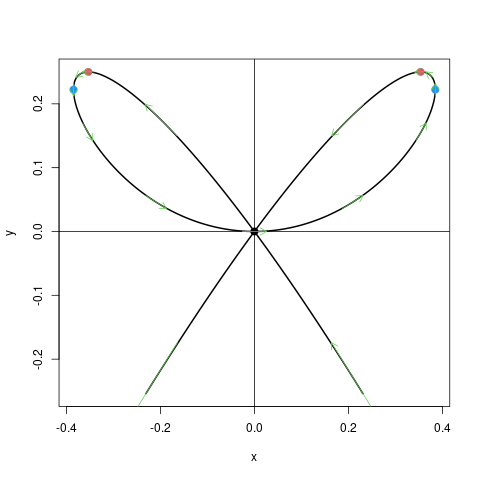
\includegraphics[width=.5\textwidth]{CourbeParametreeDim2}
    $$
  \end{description}

}
